\documentclass{standalone}
\usepackage{tikz}
\usetikzlibrary{patterns, positioning}

\begin{document}
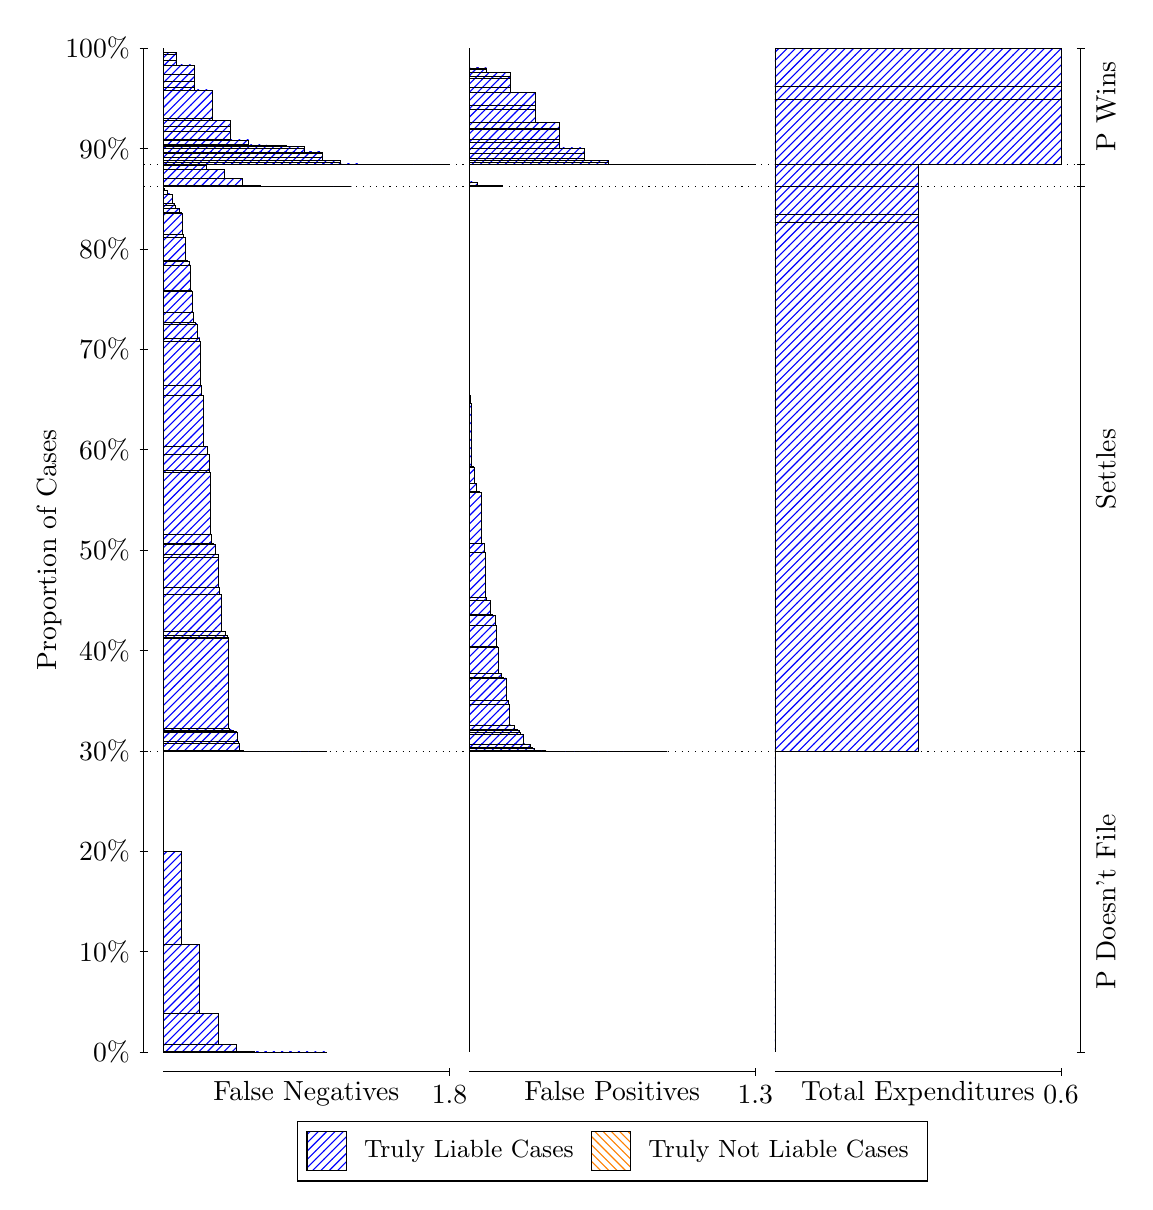
\begin{tikzpicture}
\draw[black, very thin] (1.5,1.75) -- (1.5,14.5);
\node[rotate=90, anchor=center] at (0.3, 8.125) {Proportion of Cases};
\draw[black, very thin] (1.45,1.75) -- (1.55,1.75);
\node[anchor=east] at (1.45, 1.75) {0\%};
\draw[black, very thin] (1.45,3.025) -- (1.55,3.025);
\node[anchor=east] at (1.45, 3.025) {10\%};
\draw[black, very thin] (1.45,4.3) -- (1.55,4.3);
\node[anchor=east] at (1.45, 4.3) {20\%};
\draw[black, very thin] (1.45,5.575) -- (1.55,5.575);
\node[anchor=east] at (1.45, 5.575) {30\%};
\draw[black, very thin] (1.45,6.85) -- (1.55,6.85);
\node[anchor=east] at (1.45, 6.85) {40\%};
\draw[black, very thin] (1.45,8.125) -- (1.55,8.125);
\node[anchor=east] at (1.45, 8.125) {50\%};
\draw[black, very thin] (1.45,9.4) -- (1.55,9.4);
\node[anchor=east] at (1.45, 9.4) {60\%};
\draw[black, very thin] (1.45,10.675) -- (1.55,10.675);
\node[anchor=east] at (1.45, 10.675) {70\%};
\draw[black, very thin] (1.45,11.95) -- (1.55,11.95);
\node[anchor=east] at (1.45, 11.95) {80\%};
\draw[black, very thin] (1.45,13.225) -- (1.55,13.225);
\node[anchor=east] at (1.45, 13.225) {90\%};
\draw[black, very thin] (1.45,14.5) -- (1.55,14.5);
\node[anchor=east] at (1.45, 14.5) {100\%};

\draw[black, very thin] (13.4,1.75) -- (13.4,14.5);
\draw[black, very thin] (13.35,1.75) -- (13.45,1.75);
\node[anchor=west] at (13.35, 1.75) {};
\draw[black, very thin] (13.35,5.563) -- (13.45,5.563);
\node[anchor=west] at (13.35, 5.563) {};
\draw[black, very thin] (13.35,12.743) -- (13.45,12.743);
\node[anchor=west] at (13.35, 12.743) {};
\draw[black, very thin] (13.35,13.018) -- (13.45,13.018);
\node[anchor=west] at (13.35, 13.018) {};
\draw[black, very thin] (13.35,14.5) -- (13.45,14.5);
\node[anchor=west] at (13.35, 14.5) {};

\draw[black, very thin, pattern color=blue, pattern=north east lines] (1.75,1.75) rectangle (3.8262,1.75);
\draw[black, very thin, pattern color=blue, pattern=north east lines] (1.75,1.75) rectangle (3.5955,1.75);
\draw[black, very thin, pattern color=blue, pattern=north east lines] (1.75,1.75) rectangle (3.3648,1.75);
\draw[black, very thin, pattern color=blue, pattern=north east lines] (1.75,1.75) rectangle (3.1341,1.7503);
\draw[black, very thin, pattern color=blue, pattern=north east lines] (1.75,1.7503) rectangle (2.9034,1.7582);
\draw[black, very thin, pattern color=blue, pattern=north east lines] (1.75,1.7582) rectangle (2.6728,1.8434);
\draw[black, very thin, pattern color=blue, pattern=north east lines] (1.75,1.8434) rectangle (2.4421,2.2366);
\draw[black, very thin, pattern color=blue, pattern=north east lines] (1.75,2.2366) rectangle (2.2114,3.1157);
\draw[black, very thin, pattern color=blue, pattern=north east lines] (1.75,3.1157) rectangle (1.9807,4.2995);
\draw[black, very thin, pattern color=orange, pattern=north west lines] (1.75,4.2995) rectangle (1.75,4.2995);
\draw[black, very thin, pattern color=blue, pattern=north east lines] (1.75,4.2995) rectangle (1.75,5.563);
\draw[black, very thin, pattern color=blue, pattern=north east lines] (1.75,5.563) rectangle (3.8262,5.563);
\draw[black, very thin, pattern color=blue, pattern=north east lines] (1.75,5.563) rectangle (3.7224,5.563);
\draw[black, very thin, pattern color=blue, pattern=north east lines] (1.75,5.563) rectangle (3.6186,5.563);
\draw[black, very thin, pattern color=blue, pattern=north east lines] (1.75,5.563) rectangle (3.5955,5.563);
\draw[black, very thin, pattern color=blue, pattern=north east lines] (1.75,5.563) rectangle (3.5148,5.563);
\draw[black, very thin, pattern color=blue, pattern=north east lines] (1.75,5.563) rectangle (3.4917,5.563);
\draw[black, very thin, pattern color=blue, pattern=north east lines] (1.75,5.563) rectangle (3.411,5.563);
\draw[black, very thin, pattern color=blue, pattern=north east lines] (1.75,5.563) rectangle (3.3879,5.563);
\draw[black, very thin, pattern color=blue, pattern=north east lines] (1.75,5.563) rectangle (3.3648,5.563);
\draw[black, very thin, pattern color=blue, pattern=north east lines] (1.75,5.563) rectangle (3.3071,5.563);
\draw[black, very thin, pattern color=blue, pattern=north east lines] (1.75,5.563) rectangle (3.2841,5.563);
\draw[black, very thin, pattern color=blue, pattern=north east lines] (1.75,5.563) rectangle (3.261,5.563);
\draw[black, very thin, pattern color=blue, pattern=north east lines] (1.75,5.563) rectangle (3.2033,5.563);
\draw[black, very thin, pattern color=blue, pattern=north east lines] (1.75,5.563) rectangle (3.1803,5.5631);
\draw[black, very thin, pattern color=blue, pattern=north east lines] (1.75,5.5631) rectangle (3.1572,5.5631);
\draw[black, very thin, pattern color=blue, pattern=north east lines] (1.75,5.5631) rectangle (3.1341,5.5631);
\draw[black, very thin, pattern color=blue, pattern=north east lines] (1.75,5.5631) rectangle (3.0995,5.5631);
\draw[black, very thin, pattern color=blue, pattern=north east lines] (1.75,5.5631) rectangle (3.0765,5.5631);
\draw[black, very thin, pattern color=blue, pattern=north east lines] (1.75,5.5631) rectangle (3.0534,5.5631);
\draw[black, very thin, pattern color=blue, pattern=north east lines] (1.75,5.5631) rectangle (3.0303,5.5631);
\draw[black, very thin, pattern color=blue, pattern=north east lines] (1.75,5.5631) rectangle (2.9957,5.5634);
\draw[black, very thin, pattern color=blue, pattern=north east lines] (1.75,5.5634) rectangle (2.9726,5.5634);
\draw[black, very thin, pattern color=blue, pattern=north east lines] (1.75,5.5634) rectangle (2.9496,5.5679);
\draw[black, very thin, pattern color=blue, pattern=north east lines] (1.75,5.5679) rectangle (2.9265,5.5687);
\draw[black, very thin, pattern color=blue, pattern=north east lines] (1.75,5.5687) rectangle (2.9034,5.5688);
\draw[black, very thin, pattern color=blue, pattern=north east lines] (1.75,5.5688) rectangle (2.8688,5.5692);
\draw[black, very thin, pattern color=blue, pattern=north east lines] (1.75,5.5692) rectangle (2.8458,5.5695);
\draw[black, very thin, pattern color=blue, pattern=north east lines] (1.75,5.5695) rectangle (2.8227,5.5705);
\draw[black, very thin, pattern color=blue, pattern=north east lines] (1.75,5.5705) rectangle (2.7996,5.5709);
\draw[black, very thin, pattern color=blue, pattern=north east lines] (1.75,5.5709) rectangle (2.7881,5.572);
\draw[black, very thin, pattern color=blue, pattern=north east lines] (1.75,5.572) rectangle (2.765,5.5784);
\draw[black, very thin, pattern color=blue, pattern=north east lines] (1.75,5.5784) rectangle (2.742,5.5785);
\draw[black, very thin, pattern color=blue, pattern=north east lines] (1.75,5.5785) rectangle (2.7189,5.6751);
\draw[black, very thin, pattern color=blue, pattern=north east lines] (1.75,5.6751) rectangle (2.6958,5.6914);
\draw[black, very thin, pattern color=blue, pattern=north east lines] (1.75,5.6914) rectangle (2.6843,5.8132);
\draw[black, very thin, pattern color=blue, pattern=north east lines] (1.75,5.8132) rectangle (2.6728,5.8181);
\draw[black, very thin, pattern color=blue, pattern=north east lines] (1.75,5.8181) rectangle (2.6381,5.8354);
\draw[black, very thin, pattern color=blue, pattern=north east lines] (1.75,5.8354) rectangle (2.6151,5.8409);
\draw[black, very thin, pattern color=blue, pattern=north east lines] (1.75,5.8409) rectangle (2.592,5.8632);
\draw[black, very thin, pattern color=blue, pattern=north east lines] (1.75,5.8632) rectangle (2.5805,7.0047);
\draw[black, very thin, pattern color=blue, pattern=north east lines] (1.75,7.0047) rectangle (2.5689,7.0118);
\draw[black, very thin, pattern color=blue, pattern=north east lines] (1.75,7.0118) rectangle (2.5574,7.0387);
\draw[black, very thin, pattern color=blue, pattern=north east lines] (1.75,7.0387) rectangle (2.5343,7.0876);
\draw[black, very thin, pattern color=blue, pattern=north east lines] (1.75,7.0876) rectangle (2.5113,7.0896);
\draw[black, very thin, pattern color=blue, pattern=north east lines] (1.75,7.0896) rectangle (2.4882,7.5598);
\draw[black, very thin, pattern color=blue, pattern=north east lines] (1.75,7.5598) rectangle (2.4651,7.6462);
\draw[black, very thin, pattern color=blue, pattern=north east lines] (1.75,7.6462) rectangle (2.4536,8.0312);
\draw[black, very thin, pattern color=blue, pattern=north east lines] (1.75,8.0312) rectangle (2.4421,8.0649);
\draw[black, very thin, pattern color=blue, pattern=north east lines] (1.75,8.0649) rectangle (2.4075,8.1922);
\draw[black, very thin, pattern color=blue, pattern=north east lines] (1.75,8.1922) rectangle (2.3844,8.2141);
\draw[black, very thin, pattern color=blue, pattern=north east lines] (1.75,8.2141) rectangle (2.3613,8.3216);
\draw[black, very thin, pattern color=blue, pattern=north east lines] (1.75,8.3216) rectangle (2.3498,9.114);
\draw[black, very thin, pattern color=blue, pattern=north east lines] (1.75,9.114) rectangle (2.3383,9.1364);
\draw[black, very thin, pattern color=blue, pattern=north east lines] (1.75,9.1364) rectangle (2.3267,9.3349);
\draw[black, very thin, pattern color=blue, pattern=north east lines] (1.75,9.3349) rectangle (2.3037,9.4366);
\draw[black, very thin, pattern color=blue, pattern=north east lines] (1.75,9.4366) rectangle (2.2806,9.4463);
\draw[black, very thin, pattern color=blue, pattern=north east lines] (1.75,9.4463) rectangle (2.2575,10.095);
\draw[black, very thin, pattern color=blue, pattern=north east lines] (1.75,10.095) rectangle (2.2344,10.216);
\draw[black, very thin, pattern color=blue, pattern=north east lines] (1.75,10.216) rectangle (2.2229,10.778);
\draw[black, very thin, pattern color=blue, pattern=north east lines] (1.75,10.778) rectangle (2.2114,10.819);
\draw[black, very thin, pattern color=blue, pattern=north east lines] (1.75,10.819) rectangle (2.1768,10.997);
\draw[black, very thin, pattern color=blue, pattern=north east lines] (1.75,10.997) rectangle (2.1537,11.014);
\draw[black, very thin, pattern color=blue, pattern=north east lines] (1.75,11.014) rectangle (2.1306,11.139);
\draw[black, very thin, pattern color=blue, pattern=north east lines] (1.75,11.139) rectangle (2.1191,11.406);
\draw[black, very thin, pattern color=blue, pattern=north east lines] (1.75,11.406) rectangle (2.1076,11.42);
\draw[black, very thin, pattern color=blue, pattern=north east lines] (1.75,11.42) rectangle (2.096,11.747);
\draw[black, very thin, pattern color=blue, pattern=north east lines] (1.75,11.747) rectangle (2.073,11.796);
\draw[black, very thin, pattern color=blue, pattern=north east lines] (1.75,11.796) rectangle (2.0499,11.805);
\draw[black, very thin, pattern color=blue, pattern=north east lines] (1.75,11.805) rectangle (2.0268,12.095);
\draw[black, very thin, pattern color=blue, pattern=north east lines] (1.75,12.095) rectangle (2.0038,12.138);
\draw[black, very thin, pattern color=blue, pattern=north east lines] (1.75,12.138) rectangle (1.9922,12.402);
\draw[black, very thin, pattern color=blue, pattern=north east lines] (1.75,12.402) rectangle (1.9807,12.412);
\draw[black, very thin, pattern color=blue, pattern=north east lines] (1.75,12.412) rectangle (1.9461,12.462);
\draw[black, very thin, pattern color=blue, pattern=north east lines] (1.75,12.462) rectangle (1.923,12.465);
\draw[black, very thin, pattern color=blue, pattern=north east lines] (1.75,12.465) rectangle (1.8999,12.499);
\draw[black, very thin, pattern color=blue, pattern=north east lines] (1.75,12.499) rectangle (1.8884,12.525);
\draw[black, very thin, pattern color=blue, pattern=north east lines] (1.75,12.525) rectangle (1.8769,12.527);
\draw[black, very thin, pattern color=blue, pattern=north east lines] (1.75,12.527) rectangle (1.8653,12.642);
\draw[black, very thin, pattern color=blue, pattern=north east lines] (1.75,12.642) rectangle (1.8423,12.647);
\draw[black, very thin, pattern color=blue, pattern=north east lines] (1.75,12.647) rectangle (1.8192,12.648);
\draw[black, very thin, pattern color=blue, pattern=north east lines] (1.75,12.648) rectangle (1.7961,12.689);
\draw[black, very thin, pattern color=blue, pattern=north east lines] (1.75,12.689) rectangle (1.7731,12.693);
\draw[black, very thin, pattern color=blue, pattern=north east lines] (1.75,12.693) rectangle (1.7615,12.725);
\draw[black, very thin, pattern color=orange, pattern=north west lines] (1.75,12.725) rectangle (1.75,12.725);
\draw[black, very thin, pattern color=blue, pattern=north east lines] (1.75,12.725) rectangle (1.75,12.743);
\draw[black, very thin, pattern color=blue, pattern=north east lines] (1.75,12.743) rectangle (4.1376,12.743);
\draw[black, very thin, pattern color=blue, pattern=north east lines] (1.75,12.743) rectangle (3.9069,12.743);
\draw[black, very thin, pattern color=blue, pattern=north east lines] (1.75,12.743) rectangle (3.6762,12.743);
\draw[black, very thin, pattern color=blue, pattern=north east lines] (1.75,12.743) rectangle (3.4456,12.743);
\draw[black, very thin, pattern color=blue, pattern=north east lines] (1.75,12.743) rectangle (3.2149,12.743);
\draw[black, very thin, pattern color=blue, pattern=north east lines] (1.75,12.743) rectangle (2.9842,12.757);
\draw[black, very thin, pattern color=blue, pattern=north east lines] (1.75,12.757) rectangle (2.7535,12.841);
\draw[black, very thin, pattern color=blue, pattern=north east lines] (1.75,12.841) rectangle (2.5228,12.962);
\draw[black, very thin, pattern color=blue, pattern=north east lines] (1.75,12.962) rectangle (2.2921,13.01);
\draw[black, very thin, pattern color=blue, pattern=north east lines] (1.75,13.01) rectangle (2.0614,13.018);
\draw[black, very thin, pattern color=orange, pattern=north west lines] (1.75,13.018) rectangle (1.75,13.018);
\draw[black, very thin, pattern color=blue, pattern=north east lines] (1.75,13.018) rectangle (5.3833,13.018);
\draw[black, very thin, pattern color=blue, pattern=north east lines] (1.75,13.018) rectangle (5.1526,13.018);
\draw[black, very thin, pattern color=blue, pattern=north east lines] (1.75,13.018) rectangle (4.922,13.018);
\draw[black, very thin, pattern color=blue, pattern=north east lines] (1.75,13.018) rectangle (4.6913,13.018);
\draw[black, very thin, pattern color=blue, pattern=north east lines] (1.75,13.018) rectangle (4.6913,13.018);
\draw[black, very thin, pattern color=blue, pattern=north east lines] (1.75,13.018) rectangle (4.4606,13.019);
\draw[black, very thin, pattern color=blue, pattern=north east lines] (1.75,13.019) rectangle (4.4606,13.019);
\draw[black, very thin, pattern color=blue, pattern=north east lines] (1.75,13.019) rectangle (4.2299,13.029);
\draw[black, very thin, pattern color=blue, pattern=north east lines] (1.75,13.029) rectangle (4.2184,13.029);
\draw[black, very thin, pattern color=blue, pattern=north east lines] (1.75,13.029) rectangle (3.9992,13.046);
\draw[black, very thin, pattern color=blue, pattern=north east lines] (1.75,13.046) rectangle (3.9992,13.077);
\draw[black, very thin, pattern color=blue, pattern=north east lines] (1.75,13.077) rectangle (3.9877,13.077);
\draw[black, very thin, pattern color=blue, pattern=north east lines] (1.75,13.077) rectangle (3.7685,13.113);
\draw[black, very thin, pattern color=blue, pattern=north east lines] (1.75,13.113) rectangle (3.7685,13.162);
\draw[black, very thin, pattern color=blue, pattern=north east lines] (1.75,13.162) rectangle (3.7685,13.182);
\draw[black, very thin, pattern color=blue, pattern=north east lines] (1.75,13.182) rectangle (3.757,13.182);
\draw[black, very thin, pattern color=blue, pattern=north east lines] (1.75,13.182) rectangle (3.757,13.182);
\draw[black, very thin, pattern color=blue, pattern=north east lines] (1.75,13.182) rectangle (3.5378,13.229);
\draw[black, very thin, pattern color=blue, pattern=north east lines] (1.75,13.229) rectangle (3.5378,13.253);
\draw[black, very thin, pattern color=blue, pattern=north east lines] (1.75,13.253) rectangle (3.5263,13.253);
\draw[black, very thin, pattern color=blue, pattern=north east lines] (1.75,13.253) rectangle (3.5263,13.253);
\draw[black, very thin, pattern color=blue, pattern=north east lines] (1.75,13.253) rectangle (3.3071,13.265);
\draw[black, very thin, pattern color=blue, pattern=north east lines] (1.75,13.265) rectangle (3.2956,13.266);
\draw[black, very thin, pattern color=blue, pattern=north east lines] (1.75,13.266) rectangle (3.0765,13.266);
\draw[black, very thin, pattern color=blue, pattern=north east lines] (1.75,13.266) rectangle (3.0649,13.27);
\draw[black, very thin, pattern color=blue, pattern=north east lines] (1.75,13.27) rectangle (2.8458,13.27);
\draw[black, very thin, pattern color=blue, pattern=north east lines] (1.75,13.27) rectangle (2.8458,13.27);
\draw[black, very thin, pattern color=blue, pattern=north east lines] (1.75,13.27) rectangle (2.8342,13.273);
\draw[black, very thin, pattern color=blue, pattern=north east lines] (1.75,13.273) rectangle (2.8342,13.332);
\draw[black, very thin, pattern color=blue, pattern=north east lines] (1.75,13.332) rectangle (2.6151,13.332);
\draw[black, very thin, pattern color=blue, pattern=north east lines] (1.75,13.332) rectangle (2.6151,13.332);
\draw[black, very thin, pattern color=blue, pattern=north east lines] (1.75,13.332) rectangle (2.6035,13.335);
\draw[black, very thin, pattern color=blue, pattern=north east lines] (1.75,13.335) rectangle (2.6035,13.446);
\draw[black, very thin, pattern color=blue, pattern=north east lines] (1.75,13.446) rectangle (2.6035,13.503);
\draw[black, very thin, pattern color=blue, pattern=north east lines] (1.75,13.503) rectangle (2.6035,13.581);
\draw[black, very thin, pattern color=blue, pattern=north east lines] (1.75,13.581) rectangle (2.3844,13.581);
\draw[black, very thin, pattern color=blue, pattern=north east lines] (1.75,13.581) rectangle (2.3844,13.581);
\draw[black, very thin, pattern color=blue, pattern=north east lines] (1.75,13.581) rectangle (2.3729,13.605);
\draw[black, very thin, pattern color=blue, pattern=north east lines] (1.75,13.605) rectangle (2.3729,13.967);
\draw[black, very thin, pattern color=blue, pattern=north east lines] (1.75,13.967) rectangle (2.1537,13.967);
\draw[black, very thin, pattern color=blue, pattern=north east lines] (1.75,13.967) rectangle (2.1422,14.006);
\draw[black, very thin, pattern color=blue, pattern=north east lines] (1.75,14.006) rectangle (2.1422,14.08);
\draw[black, very thin, pattern color=blue, pattern=north east lines] (1.75,14.08) rectangle (2.1422,14.168);
\draw[black, very thin, pattern color=blue, pattern=north east lines] (1.75,14.168) rectangle (2.1422,14.285);
\draw[black, very thin, pattern color=blue, pattern=north east lines] (1.75,14.285) rectangle (1.9115,14.342);
\draw[black, very thin, pattern color=blue, pattern=north east lines] (1.75,14.342) rectangle (1.9115,14.422);
\draw[black, very thin, pattern color=blue, pattern=north east lines] (1.75,14.422) rectangle (1.9115,14.444);
\draw[black, very thin, pattern color=orange, pattern=north west lines] (1.75,14.444) rectangle (1.75,14.444);
\draw[black, very thin, pattern color=blue, pattern=north east lines] (1.75,14.444) rectangle (1.75,14.5);
\draw[black, very thin, pattern color=orange, pattern=north west lines] (5.6333,1.75) rectangle (5.6333,1.75);
\draw[black, very thin, pattern color=blue, pattern=north east lines] (5.6333,1.75) rectangle (5.6333,5.563);
\draw[black, very thin, pattern color=orange, pattern=north west lines] (5.6333,5.563) rectangle (8.1487,5.563);
\draw[black, very thin, pattern color=blue, pattern=north east lines] (5.6333,5.563) rectangle (8.1487,5.563);
\draw[black, very thin, pattern color=orange, pattern=north west lines] (5.6333,5.563) rectangle (8.009,5.563);
\draw[black, very thin, pattern color=blue, pattern=north east lines] (5.6333,5.563) rectangle (8.009,5.563);
\draw[black, very thin, pattern color=orange, pattern=north west lines] (5.6333,5.563) rectangle (7.8692,5.563);
\draw[black, very thin, pattern color=blue, pattern=north east lines] (5.6333,5.563) rectangle (7.8692,5.563);
\draw[black, very thin, pattern color=blue, pattern=north east lines] (5.6333,5.563) rectangle (7.8382,5.563);
\draw[black, very thin, pattern color=blue, pattern=north east lines] (5.6333,5.563) rectangle (7.6984,5.563);
\draw[black, very thin, pattern color=orange, pattern=north west lines] (5.6333,5.563) rectangle (7.5897,5.563);
\draw[black, very thin, pattern color=blue, pattern=north east lines] (5.6333,5.563) rectangle (7.5897,5.563);
\draw[black, very thin, pattern color=blue, pattern=north east lines] (5.6333,5.563) rectangle (7.5587,5.563);
\draw[black, very thin, pattern color=blue, pattern=north east lines] (5.6333,5.563) rectangle (7.5276,5.563);
\draw[black, very thin, pattern color=orange, pattern=north west lines] (5.6333,5.563) rectangle (7.45,5.563);
\draw[black, very thin, pattern color=blue, pattern=north east lines] (5.6333,5.563) rectangle (7.45,5.563);
\draw[black, very thin, pattern color=blue, pattern=north east lines] (5.6333,5.563) rectangle (7.3879,5.563);
\draw[black, very thin, pattern color=orange, pattern=north west lines] (5.6333,5.563) rectangle (7.3103,5.563);
\draw[black, very thin, pattern color=blue, pattern=north east lines] (5.6333,5.563) rectangle (7.3103,5.563);
\draw[black, very thin, pattern color=blue, pattern=north east lines] (5.6333,5.563) rectangle (7.2792,5.563);
\draw[black, very thin, pattern color=blue, pattern=north east lines] (5.6333,5.563) rectangle (7.2481,5.563);
\draw[black, very thin, pattern color=blue, pattern=north east lines] (5.6333,5.563) rectangle (7.2171,5.563);
\draw[black, very thin, pattern color=orange, pattern=north west lines] (5.6333,5.563) rectangle (7.1705,5.563);
\draw[black, very thin, pattern color=blue, pattern=north east lines] (5.6333,5.563) rectangle (7.1705,5.563);
\draw[black, very thin, pattern color=blue, pattern=north east lines] (5.6333,5.563) rectangle (7.1395,5.563);
\draw[black, very thin, pattern color=blue, pattern=north east lines] (5.6333,5.563) rectangle (7.0774,5.563);
\draw[black, very thin, pattern color=orange, pattern=north west lines] (5.6333,5.563) rectangle (7.0308,5.563);
\draw[black, very thin, pattern color=blue, pattern=north east lines] (5.6333,5.563) rectangle (7.0308,5.563);
\draw[black, very thin, pattern color=blue, pattern=north east lines] (5.6333,5.563) rectangle (6.9997,5.563);
\draw[black, very thin, pattern color=blue, pattern=north east lines] (5.6333,5.563) rectangle (6.9687,5.563);
\draw[black, very thin, pattern color=blue, pattern=north east lines] (5.6333,5.563) rectangle (6.9376,5.5632);
\draw[black, very thin, pattern color=blue, pattern=north east lines] (5.6333,5.5632) rectangle (6.9066,5.5632);
\draw[black, very thin, pattern color=orange, pattern=north west lines] (5.6333,5.5632) rectangle (6.891,5.5632);
\draw[black, very thin, pattern color=blue, pattern=north east lines] (5.6333,5.5632) rectangle (6.891,5.5632);
\draw[black, very thin, pattern color=blue, pattern=north east lines] (5.6333,5.5632) rectangle (6.86,5.5632);
\draw[black, very thin, pattern color=blue, pattern=north east lines] (5.6333,5.5632) rectangle (6.8289,5.5632);
\draw[black, very thin, pattern color=blue, pattern=north east lines] (5.6333,5.5632) rectangle (6.7668,5.5641);
\draw[black, very thin, pattern color=orange, pattern=north west lines] (5.6333,5.5641) rectangle (6.7513,5.5641);
\draw[black, very thin, pattern color=blue, pattern=north east lines] (5.6333,5.5641) rectangle (6.7513,5.5643);
\draw[black, very thin, pattern color=blue, pattern=north east lines] (5.6333,5.5643) rectangle (6.7202,5.5659);
\draw[black, very thin, pattern color=blue, pattern=north east lines] (5.6333,5.5659) rectangle (6.6892,5.5659);
\draw[black, very thin, pattern color=blue, pattern=north east lines] (5.6333,5.5659) rectangle (6.6581,5.566);
\draw[black, very thin, pattern color=blue, pattern=north east lines] (5.6333,5.566) rectangle (6.6271,5.5747);
\draw[black, very thin, pattern color=orange, pattern=north west lines] (5.6333,5.5747) rectangle (6.6115,5.5747);
\draw[black, very thin, pattern color=blue, pattern=north east lines] (5.6333,5.5747) rectangle (6.6115,5.5747);
\draw[black, very thin, pattern color=blue, pattern=north east lines] (5.6333,5.5747) rectangle (6.596,5.5753);
\draw[black, very thin, pattern color=blue, pattern=north east lines] (5.6333,5.5753) rectangle (6.5805,5.5773);
\draw[black, very thin, pattern color=blue, pattern=north east lines] (5.6333,5.5773) rectangle (6.5494,5.5773);
\draw[black, very thin, pattern color=blue, pattern=north east lines] (5.6333,5.5773) rectangle (6.5184,5.5803);
\draw[black, very thin, pattern color=orange, pattern=north west lines] (5.6333,5.5803) rectangle (6.4718,5.5803);
\draw[black, very thin, pattern color=blue, pattern=north east lines] (5.6333,5.5803) rectangle (6.4718,5.5812);
\draw[black, very thin, pattern color=blue, pattern=north east lines] (5.6333,5.5812) rectangle (6.4563,5.613);
\draw[black, very thin, pattern color=blue, pattern=north east lines] (5.6333,5.613) rectangle (6.4407,5.617);
\draw[black, very thin, pattern color=blue, pattern=north east lines] (5.6333,5.617) rectangle (6.4097,5.6574);
\draw[black, very thin, pattern color=blue, pattern=north east lines] (5.6333,5.6574) rectangle (6.3786,5.6587);
\draw[black, very thin, pattern color=blue, pattern=north east lines] (5.6333,5.6587) rectangle (6.3476,5.6638);
\draw[black, very thin, pattern color=blue, pattern=north east lines] (5.6333,5.6638) rectangle (6.3165,5.7791);
\draw[black, very thin, pattern color=blue, pattern=north east lines] (5.6333,5.7791) rectangle (6.301,5.7809);
\draw[black, very thin, pattern color=blue, pattern=north east lines] (5.6333,5.7809) rectangle (6.2855,5.8071);
\draw[black, very thin, pattern color=blue, pattern=north east lines] (5.6333,5.8071) rectangle (6.2699,5.8407);
\draw[black, very thin, pattern color=blue, pattern=north east lines] (5.6333,5.8407) rectangle (6.2389,5.8434);
\draw[black, very thin, pattern color=blue, pattern=north east lines] (5.6333,5.8434) rectangle (6.2078,5.8936);
\draw[black, very thin, pattern color=blue, pattern=north east lines] (5.6333,5.8936) rectangle (6.1613,5.9041);
\draw[black, very thin, pattern color=blue, pattern=north east lines] (5.6333,5.9041) rectangle (6.1457,6.1676);
\draw[black, very thin, pattern color=blue, pattern=north east lines] (5.6333,6.1676) rectangle (6.1302,6.2109);
\draw[black, very thin, pattern color=blue, pattern=north east lines] (5.6333,6.2109) rectangle (6.0991,6.5012);
\draw[black, very thin, pattern color=blue, pattern=north east lines] (5.6333,6.5012) rectangle (6.0681,6.5099);
\draw[black, very thin, pattern color=blue, pattern=north east lines] (5.6333,6.5099) rectangle (6.037,6.5583);
\draw[black, very thin, pattern color=blue, pattern=north east lines] (5.6333,6.5583) rectangle (6.006,6.8855);
\draw[black, very thin, pattern color=blue, pattern=north east lines] (5.6333,6.8855) rectangle (5.9905,6.8993);
\draw[black, very thin, pattern color=blue, pattern=north east lines] (5.6333,6.8993) rectangle (5.9749,7.1668);
\draw[black, very thin, pattern color=blue, pattern=north east lines] (5.6333,7.1668) rectangle (5.9594,7.2918);
\draw[black, very thin, pattern color=blue, pattern=north east lines] (5.6333,7.2918) rectangle (5.9283,7.3091);
\draw[black, very thin, pattern color=blue, pattern=north east lines] (5.6333,7.3091) rectangle (5.8973,7.4864);
\draw[black, very thin, pattern color=blue, pattern=north east lines] (5.6333,7.4864) rectangle (5.8507,7.5275);
\draw[black, very thin, pattern color=blue, pattern=north east lines] (5.6333,7.5275) rectangle (5.8352,8.0901);
\draw[black, very thin, pattern color=blue, pattern=north east lines] (5.6333,8.0901) rectangle (5.8197,8.2111);
\draw[black, very thin, pattern color=blue, pattern=north east lines] (5.6333,8.2111) rectangle (5.7886,8.8595);
\draw[black, very thin, pattern color=blue, pattern=north east lines] (5.6333,8.8595) rectangle (5.7575,8.8692);
\draw[black, very thin, pattern color=blue, pattern=north east lines] (5.6333,8.8692) rectangle (5.7265,8.9709);
\draw[black, very thin, pattern color=blue, pattern=north east lines] (5.6333,8.9709) rectangle (5.6954,9.1693);
\draw[black, very thin, pattern color=blue, pattern=north east lines] (5.6333,9.1693) rectangle (5.6799,9.1918);
\draw[black, very thin, pattern color=blue, pattern=north east lines] (5.6333,9.1918) rectangle (5.6644,9.9841);
\draw[black, very thin, pattern color=blue, pattern=north east lines] (5.6333,9.9841) rectangle (5.6489,10.092);
\draw[black, very thin, pattern color=blue, pattern=north east lines] (5.6333,10.092) rectangle (5.6333,12.743);
\draw[black, very thin, pattern color=orange, pattern=north west lines] (5.6333,12.743) rectangle (6.0526,12.743);
\draw[black, very thin, pattern color=blue, pattern=north east lines] (5.6333,12.743) rectangle (6.0526,12.751);
\draw[black, very thin, pattern color=blue, pattern=north east lines] (5.6333,12.751) rectangle (5.742,12.799);
\draw[black, very thin, pattern color=blue, pattern=north east lines] (5.6333,12.799) rectangle (5.6333,13.018);
\draw[black, very thin, pattern color=orange, pattern=north west lines] (5.6333,13.018) rectangle (9.2667,13.018);
\draw[black, very thin, pattern color=blue, pattern=north east lines] (5.6333,13.018) rectangle (9.2667,13.018);
\draw[black, very thin, pattern color=orange, pattern=north west lines] (5.6333,13.018) rectangle (8.9561,13.018);
\draw[black, very thin, pattern color=blue, pattern=north east lines] (5.6333,13.018) rectangle (8.9561,13.018);
\draw[black, very thin, pattern color=blue, pattern=north east lines] (5.6333,13.018) rectangle (8.6456,13.018);
\draw[black, very thin, pattern color=orange, pattern=north west lines] (5.6333,13.018) rectangle (8.6456,13.018);
\draw[black, very thin, pattern color=blue, pattern=north east lines] (5.6333,13.018) rectangle (8.6456,13.018);
\draw[black, very thin, pattern color=blue, pattern=north east lines] (5.6333,13.018) rectangle (8.335,13.018);
\draw[black, very thin, pattern color=blue, pattern=north east lines] (5.6333,13.018) rectangle (8.335,13.018);
\draw[black, very thin, pattern color=orange, pattern=north west lines] (5.6333,13.018) rectangle (8.335,13.018);
\draw[black, very thin, pattern color=blue, pattern=north east lines] (5.6333,13.018) rectangle (8.335,13.018);
\draw[black, very thin, pattern color=orange, pattern=north west lines] (5.6333,13.018) rectangle (8.0245,13.018);
\draw[black, very thin, pattern color=blue, pattern=north east lines] (5.6333,13.018) rectangle (8.0245,13.018);
\draw[black, very thin, pattern color=blue, pattern=north east lines] (5.6333,13.018) rectangle (8.0245,13.019);
\draw[black, very thin, pattern color=blue, pattern=north east lines] (5.6333,13.019) rectangle (8.0245,13.019);
\draw[black, very thin, pattern color=orange, pattern=north west lines] (5.6333,13.019) rectangle (7.714,13.019);
\draw[black, very thin, pattern color=blue, pattern=north east lines] (5.6333,13.019) rectangle (7.714,13.025);
\draw[black, very thin, pattern color=blue, pattern=north east lines] (5.6333,13.025) rectangle (7.714,13.026);
\draw[black, very thin, pattern color=blue, pattern=north east lines] (5.6333,13.026) rectangle (7.4034,13.043);
\draw[black, very thin, pattern color=orange, pattern=north west lines] (5.6333,13.043) rectangle (7.4034,13.043);
\draw[black, very thin, pattern color=blue, pattern=north east lines] (5.6333,13.043) rectangle (7.4034,13.074);
\draw[black, very thin, pattern color=blue, pattern=north east lines] (5.6333,13.074) rectangle (7.0929,13.096);
\draw[black, very thin, pattern color=blue, pattern=north east lines] (5.6333,13.096) rectangle (7.0929,13.165);
\draw[black, very thin, pattern color=orange, pattern=north west lines] (5.6333,13.165) rectangle (7.0929,13.165);
\draw[black, very thin, pattern color=blue, pattern=north east lines] (5.6333,13.165) rectangle (7.0929,13.233);
\draw[black, very thin, pattern color=blue, pattern=north east lines] (5.6333,13.233) rectangle (6.7823,13.297);
\draw[black, very thin, pattern color=blue, pattern=north east lines] (5.6333,13.297) rectangle (6.7823,13.34);
\draw[black, very thin, pattern color=orange, pattern=north west lines] (5.6333,13.34) rectangle (6.7823,13.34);
\draw[black, very thin, pattern color=blue, pattern=north east lines] (5.6333,13.34) rectangle (6.7823,13.471);
\draw[black, very thin, pattern color=blue, pattern=north east lines] (5.6333,13.471) rectangle (6.7823,13.476);
\draw[black, very thin, pattern color=blue, pattern=north east lines] (5.6333,13.476) rectangle (6.7823,13.551);
\draw[black, very thin, pattern color=orange, pattern=north west lines] (5.6333,13.551) rectangle (6.7668,13.551);
\draw[black, very thin, pattern color=blue, pattern=north east lines] (5.6333,13.551) rectangle (6.7668,13.551);
\draw[black, very thin, pattern color=blue, pattern=north east lines] (5.6333,13.551) rectangle (6.4718,13.726);
\draw[black, very thin, pattern color=blue, pattern=north east lines] (5.6333,13.726) rectangle (6.4718,13.778);
\draw[black, very thin, pattern color=blue, pattern=north east lines] (5.6333,13.778) rectangle (6.4718,13.937);
\draw[black, very thin, pattern color=blue, pattern=north east lines] (5.6333,13.937) rectangle (6.4563,13.937);
\draw[black, very thin, pattern color=orange, pattern=north west lines] (5.6333,13.937) rectangle (6.4563,13.937);
\draw[black, very thin, pattern color=blue, pattern=north east lines] (5.6333,13.937) rectangle (6.4563,13.937);
\draw[black, very thin, pattern color=blue, pattern=north east lines] (5.6333,13.937) rectangle (6.1613,13.998);
\draw[black, very thin, pattern color=blue, pattern=north east lines] (5.6333,13.998) rectangle (6.1613,14.12);
\draw[black, very thin, pattern color=blue, pattern=north east lines] (5.6333,14.12) rectangle (6.1613,14.147);
\draw[black, very thin, pattern color=blue, pattern=north east lines] (5.6333,14.147) rectangle (6.1613,14.186);
\draw[black, very thin, pattern color=blue, pattern=north east lines] (5.6333,14.186) rectangle (6.1457,14.186);
\draw[black, very thin, pattern color=orange, pattern=north west lines] (5.6333,14.186) rectangle (6.1457,14.186);
\draw[black, very thin, pattern color=blue, pattern=north east lines] (5.6333,14.186) rectangle (6.1457,14.186);
\draw[black, very thin, pattern color=blue, pattern=north east lines] (5.6333,14.186) rectangle (5.8507,14.227);
\draw[black, very thin, pattern color=blue, pattern=north east lines] (5.6333,14.227) rectangle (5.8507,14.229);
\draw[black, very thin, pattern color=blue, pattern=north east lines] (5.6333,14.229) rectangle (5.8507,14.247);
\draw[black, very thin, pattern color=blue, pattern=north east lines] (5.6333,14.247) rectangle (5.8352,14.247);
\draw[black, very thin, pattern color=orange, pattern=north west lines] (5.6333,14.247) rectangle (5.8352,14.247);
\draw[black, very thin, pattern color=blue, pattern=north east lines] (5.6333,14.247) rectangle (5.8352,14.247);
\draw[black, very thin, pattern color=orange, pattern=north west lines] (5.6333,14.247) rectangle (5.6333,14.247);
\draw[black, very thin, pattern color=blue, pattern=north east lines] (5.6333,14.247) rectangle (5.6333,14.5);
\draw[black, very thin, pattern color=orange, pattern=north west lines] (9.5167,1.75) rectangle (9.5167,1.75);
\draw[black, very thin, pattern color=blue, pattern=north east lines] (9.5167,1.75) rectangle (9.5167,5.563);
\draw[black, very thin, pattern color=orange, pattern=north west lines] (9.5167,5.563) rectangle (11.333,5.563);
\draw[black, very thin, pattern color=blue, pattern=north east lines] (9.5167,5.563) rectangle (11.333,12.292);
\draw[black, very thin, pattern color=orange, pattern=north west lines] (9.5167,12.292) rectangle (11.333,12.292);
\draw[black, very thin, pattern color=blue, pattern=north east lines] (9.5167,12.292) rectangle (11.333,12.384);
\draw[black, very thin, pattern color=orange, pattern=north west lines] (9.5167,12.384) rectangle (11.333,12.384);
\draw[black, very thin, pattern color=blue, pattern=north east lines] (9.5167,12.384) rectangle (11.333,12.743);
\draw[black, very thin, pattern color=orange, pattern=north west lines] (9.5167,12.743) rectangle (11.333,12.743);
\draw[black, very thin, pattern color=blue, pattern=north east lines] (9.5167,12.743) rectangle (11.333,13.018);
\draw[black, very thin, pattern color=orange, pattern=north west lines] (9.5167,13.018) rectangle (13.15,13.018);
\draw[black, very thin, pattern color=blue, pattern=north east lines] (9.5167,13.018) rectangle (13.15,13.843);
\draw[black, very thin, pattern color=orange, pattern=north west lines] (9.5167,13.843) rectangle (13.15,13.843);
\draw[black, very thin, pattern color=blue, pattern=north east lines] (9.5167,13.843) rectangle (13.15,14.01);
\draw[black, very thin, pattern color=orange, pattern=north west lines] (9.5167,14.01) rectangle (13.15,14.01);
\draw[black, very thin, pattern color=blue, pattern=north east lines] (9.5167,14.01) rectangle (13.15,14.5);
\draw[black, dotted] (1.5,5.563) -- (13.4,5.563);
\draw[black, dotted] (1.5,12.743) -- (13.4,12.743);
\draw[black, dotted] (1.5,13.018) -- (13.4,13.018);
\draw[black, very thin] (1.75,1.5) -- (5.3833,1.5);
\node[anchor=north] at (3.5667, 1.5) {False Negatives};
\draw[black, very thin] (5.3833,1.45) -- (5.3833,1.55);
\node[anchor=north] at (5.3833, 1.45) {1.8};

\draw[black, very thin] (5.6333,1.5) -- (9.2667,1.5);
\node[anchor=north] at (7.45, 1.5) {False Positives};
\draw[black, very thin] (9.2667,1.45) -- (9.2667,1.55);
\node[anchor=north] at (9.2667, 1.45) {1.3};

\draw[black, very thin] (9.5167,1.5) -- (13.15,1.5);
\node[anchor=north] at (11.333, 1.5) {Total Expenditures};
\draw[black, very thin] (13.15,1.45) -- (13.15,1.55);
\node[anchor=north] at (13.15, 1.45) {0.6};

\node[black, centered, rotate=90] at (13.72, 3.6565) {P Doesn't File};
\node[black, centered, rotate=90] at (13.72, 9.1529) {Settles};

\node[black, centered, rotate=90] at (13.72, 13.759) {P Wins};

\draw (7.449999999999999,1.5) node[draw=none] (baseCoordinate) {};
\begin{scope}[align=center]
        \matrix[scale=0.5, draw=black, below=0.5cm of baseCoordinate, nodes={draw}, column sep=0.1cm]{
            \node[rectangle, draw, minimum width=0.5cm, minimum height=0.5cm, pattern=north east lines, pattern color=blue] {}; &
            \node[draw=none, font=\small] (B) {Truly Liable Cases}; &
            \node[rectangle, draw, minimum width=0.5cm, minimum height=0.5cm, pattern=north west lines, pattern color=orange] {}; &
            \node[draw=none, font=\small] (B) {Truly Not Liable Cases}; \\
            };
\end{scope}

\end{tikzpicture}
\end{document}